\chapter{Datasets}
\label{chap:datasets}

\section{TREC 2019 - Deep Learning Track}
\label{sec:trec2019}
The TREC 2019 deep learning track focuses on studying text retrieval on large-scale data \cite{DBLP:journals/corr/abs-2003-07820}. It provides two datasets, one for passage retrieval and one for document retrieval. The datasets are based on MS MARCO \cite{DBLP:journals/corr/NguyenRSGTMD16} which consists of $\sim 1$mio real world user queries from the Bing search engine and a corpus of $\sim 8.8$mio passages. The passages in the passage dataset are extracted from the document dataset, hence there can be multiple passages for each document. Because of this, the document dataset contains less than half the number of samples.

Since the models we study in this thesis are limited in input length, we will focus on the passage retrieval dataset (TREC2019) if not stated otherwise. Further, we will refer to passages from this dataset as documents, to be consistent with the common information retrieval terminology.
\begin{table}[h]
    \centering
    \begin{tabular}{c|ccc}
        \hline
        \tf{Dataset} & \tf{Train} & \tf{Validation} & \tf{Test} \\ \hline\hline
        Passage      & 502,939    & 55,578          & 200       \\ \hline
        Document     & 367,013    & 5,193           & 200       \\ \hline
    \end{tabular}
    \caption{Number of queries for each dataset split in the two TREC 2019 datasets.}
\end{table}
\begin{table}[h]
    \centering

    \begin{tabular}{c|c}
        \hline
        \tf{Passage} & \tf{Document} \\ \hline\hline
        8,841,823    & 3,213,835     \\ \hline
    \end{tabular}
    \caption{Corpus size for each TREC dataset.}
\end{table}

While with TREC2019, two types of tasks are provided, namely full ranking and re-ranking, we will only perform the re-ranking task. This means, given a pool of $1000$ documents for each query, we need to provide an ordering, such that relevant documents are placed at the top. On average, a query has $\sim 1.1$ relevant documents in its pool which were marked as relevant by human annotators. Note that each annotator only had access to $\sim 10$ passages during annotation, meaning a pool is likely to contain false negatives, i.e. relevant passages that are not marked as such.

Opposed to this, documents in the document dataset are automatically marked as relevant, if they contain at least $1$ relevant passage.

\section{Probing Dataset Generation}
\label{sec:dataset_gen}
For all of our probing tasks (\autoref{sec:tasks}), we automatically generate datasets from the TREC2019 passage-level test set. To achieve this, we sample $60$k query-document pairs from the test set of which $40$k are used as training set and $10$k as validation and test set, respectively. We then use existing tools to extract the properties that we are interested in and use them to label the data. Details on how we generate labels for each task are described in \autoref{sec:tasks}. Examples for each task are shown in \autoref{tab:data_examples}. Throughout this thesis, we will abbreviate each task name as follows: Semantic similarity (SEM), named entity recognition (NER), coreference (COREF), fact checking (FACT).

\begin{table}
    \centering
    \begin{tabular}{l|p{0.2\textwidth}|p{0.4\textwidth}|c}
        \hline
        \tf{Task} & \tf{Query}                                                 & \tf{Document}                                                                                                                                                       & \tf{Target}  \\ \hline\hline
        BM25      & how many days to defrost                                   & The best way to safely and quickly defrost chicken, he says, is\dots                                                                                                & 11.44        \\ \hline
        SEM       & how many of grams a sugar should a person have in one day? & According to the Institute of Medicine, Food and Nutrition Board, the average person needs 0.32 grams of protein per pound of body weight\dots                      & 0.316        \\ \hline
        NER       & what company was skittles made by?                         & \tf{[Wrigley]} is a company that makes and sells gum, hard candies, and lollipops\dots                                                                              & Organization \\ \hline
        COREF     & at what age do \tf{[kittens]} get their first shots        & Kittens this age will begin to eat regular cat food, and will begin to use a litter box. \tf{[They]} are still quite small at this age\dots                         & True         \\ \hline
        FACT      & Big Brother 18 is hosted by Emma Willis.                   & Big Brother 2017, also known as Big Brother 18, is the upcoming eighteenth series of the British reality television series Big Brother, hosted by Emma Willis \dots & Supports     \\ \hline
    \end{tabular}
    \caption{Training examples from each probing dataset and their respective targets. Target spans within the text are highlighted in square brackets.}
    \label{tab:data_examples}
\end{table}

\begin{figure}
    \centering
    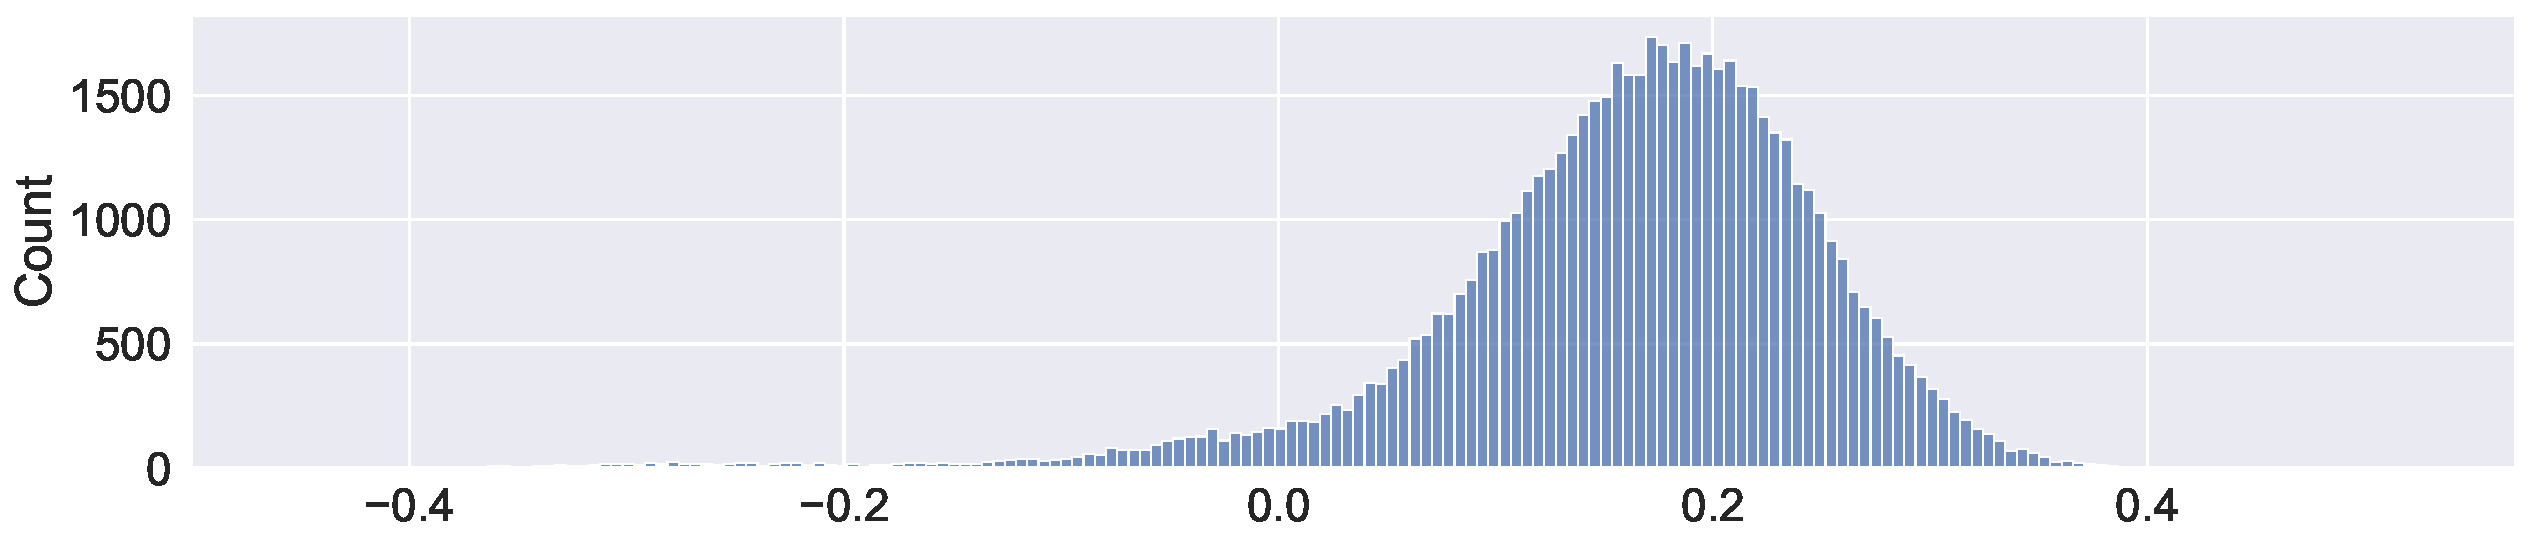
\includegraphics[width=\textwidth]{gfx/probing/labels/sem}
    \caption{Distribution of SEM target scores.}

    \bigskip

    \centering
    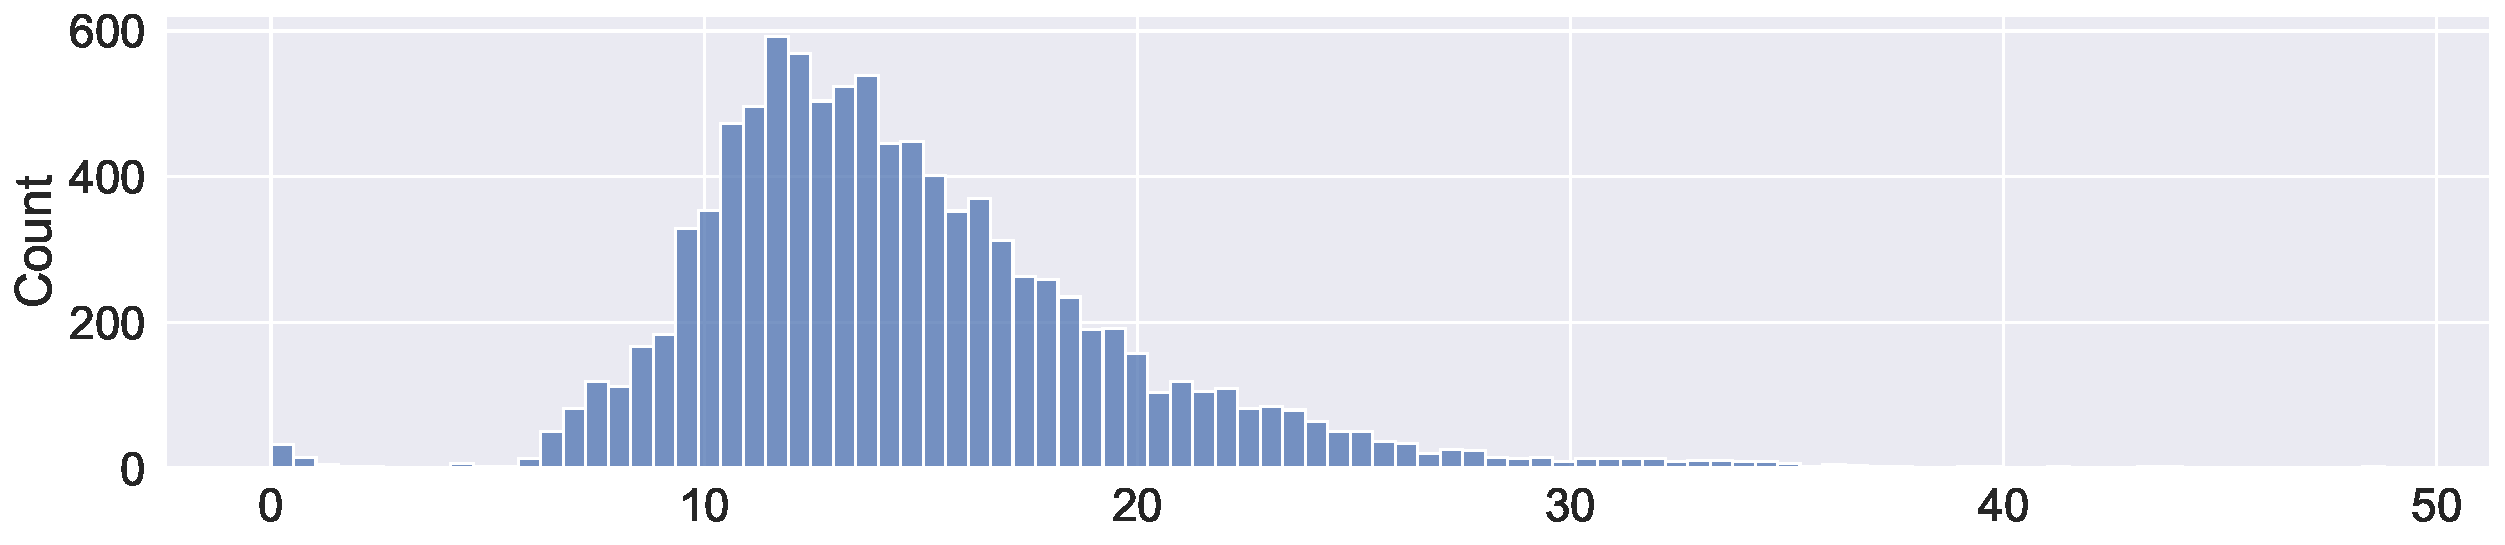
\includegraphics[width=\textwidth]{gfx/probing/labels/bm25}
    \caption{Distribution of BM25 target scores.}

    \bigskip

    \centering
    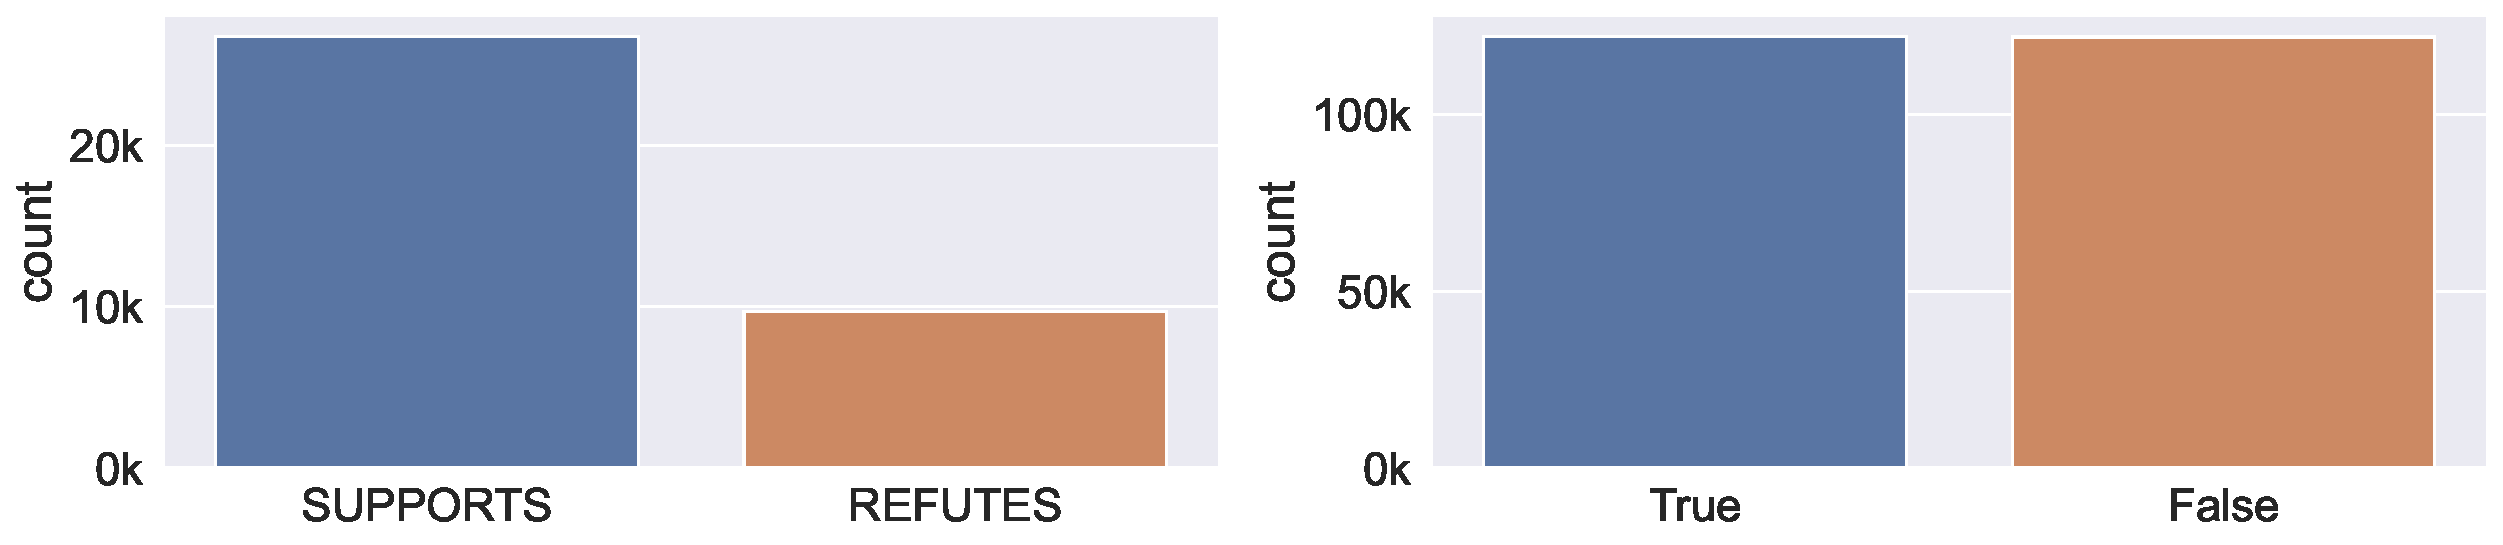
\includegraphics[width=\textwidth]{gfx/probing/labels/fever_coref}
    \caption{Distribution of FEVER and COREF labels. COREF negatives are sampled for each positive.}

    \bigskip

    \centering
    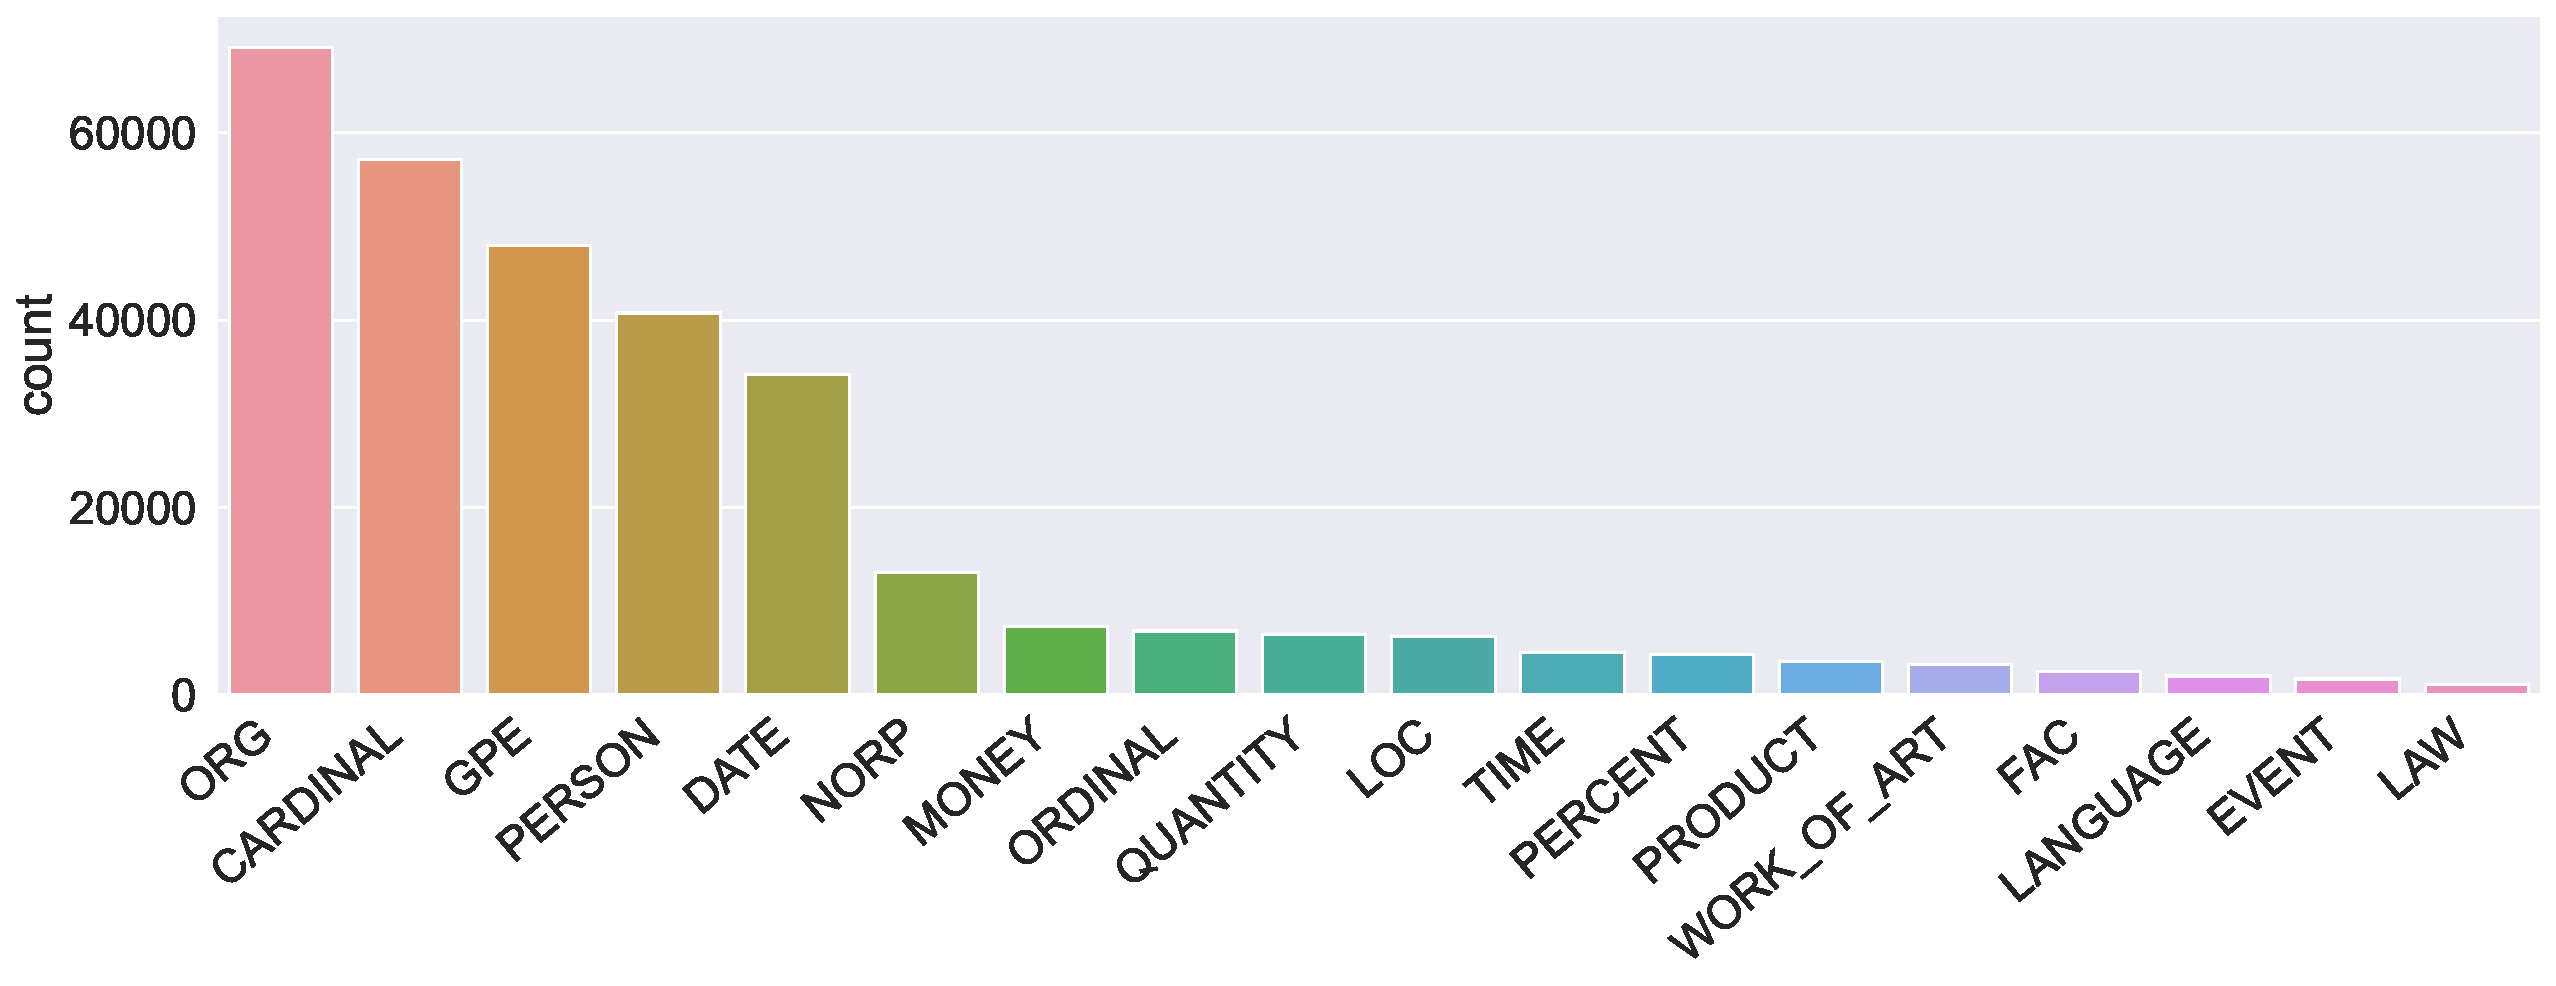
\includegraphics[width=\textwidth]{gfx/probing/labels/ner}
    \caption{Distribution of named entity types in the NER dataset.}

\end{figure}
